\documentclass[11pt, a4paper]{article}

\usepackage[utf8]{inputenc}
\usepackage[a4paper, total={6in, 8in}]{geometry}
\raggedbottom

\usepackage{mlmodern}
\usepackage{csquotes}
\usepackage{parskip}
\usepackage[italian]{babel}
\usepackage{booktabs}
\usepackage{multicol}
\usepackage{graphicx}
\usepackage{fancyhdr}
\usepackage{float}
\usepackage{changepage}
\usepackage{fancyvrb}
\usepackage[final]{pdfpages}
\usepackage{placeins}
\usepackage{hyperref}
\usepackage[all]{hypcap}
\usepackage{tcolorbox}
\usepackage{xurl}
\usepackage{xcolor}
\usepackage{tikz}
\usepackage{biblatex}
\usepackage{array}
\usepackage{pdfpages}
\usepackage{subfig}
\usepackage{multirow}
\usepackage{pgfplots}
\usepackage{listings}
\usepackage{subfig}
\usepackage{caption}
\usepackage{pdfpages}
\usepackage{placeins}
\usepackage{listings}
\usepgfplotslibrary{groupplots}
\pgfplotsset{compat=1.18}

\lstset{
	language=C++,
	tabsize=4,
	keepspaces,
	extendedchars=true,
	rulecolor=\color{black},
	basicstyle=\footnotesize,
	aboveskip=5pt,
	upquote=true,
	columns=fixed,
	showstringspaces=false,
	extendedchars=true,
	breaklines=false,
	frame=single,
	showtabs=false,
	showspaces=false,
	showstringspaces=false,
}


\addbibresource{bibliography.bib}

\hypersetup{
	colorlinks=false,
	citecolor=black,
	filecolor=black,
	linkcolor=black,
	urlcolor=black,
	allbordercolors=white
}


\definecolor{codegreen}{rgb}{0,0.6,0}
\definecolor{codegray}{rgb}{0.5,0.5,0.5}
\definecolor{codepurple}{rgb}{0.58,0,0.82}
\definecolor{backcolour}{rgb}{0.95,0.95,0.92}

\lstdefinestyle{mystyle}{
	backgroundcolor=\color{backcolour},   
	commentstyle=\color{codegreen},
	numberstyle=\tiny\color{codegray},
	stringstyle=\color{codepurple},
	basicstyle=\ttfamily\footnotesize,
	breakatwhitespace=false,         
	breaklines=true,                 
	captionpos=b,                    
	keepspaces=true,                   
	numbersep=5pt,                  
	showspaces=false,                
	showstringspaces=false,
	showtabs=false,                  
	tabsize=1
}

\lstset{style=mystyle}



\setlength{\headheight}{14pt}

\begin{document}
	\begin{center}
	{\LARGE \textbf{Università degli Studi di Milano Bicocca}} \\
	\vspace{0.2cm}
	{\Large {Dipartimento di Informatica}} \\ 
	\vspace{1cm}
	
	
\includegraphics[width=4cm]{figures/unimib-logo.png} \\
	\vspace{0.4cm}
	
	{\huge \textbf{Metodi del calcolo scientifico}} \\ 
	\Large{Libreria MatrixDestoryer per la risoluzione di sistemi lineari in modo iterativi}
	\vspace{1cm}
\end{center}
\vspace{2cm}

\noindent \large{Membri del gruppo:} 

\begin{tabular}{@{}lll}
	\textbf{Canesi Gabriele} & 851637 & \href{mailto:g.canesi1@campus.unimib.it}{\texttt{g.canesi1@campus.unimib.it}}\\
	\textbf{Fiorenza Gioele} & 851631 & \href{mailto:g.fiorenza1@campus.unimib.it}{\texttt{g.fiorenza1@campus.unimib.it}}\\
	\textbf{Ghislotti Gianluca} & 859242 & \href{mailto:g.ghislotti@campus.unimib.it}{\texttt{g.ghislotti@campus.unimib.it}}\\
\end{tabular}

\vfill
\begin{center}
	\large{\textbf{Anno Accademico 2023/2024}}
\end{center}




	\thispagestyle{empty}
	\newpage
	\pagestyle{fancy}
	\pagenumbering{roman}
	
	
	\tableofcontents
	
	\newpage
	
	\definecolor{fireenginered}{rgb}{0.81, 0.09, 0.13}
	\hypersetup{
		linkbordercolor=fireenginered
	}
	\pagenumbering{arabic}
	
	\section{Introduzione}

La risoluzione di sistemi lineari può diventare rapidamente onerosa, in termini di memoria e operazioni, nel caso in cui le matrici in input siano sparse. Ciò è dovuto al fenomeno del \textbf{fill in}, ovvero la necessità di istanziare matrici dense durante la risoluzione tramite metodi diretti.

I metodi \textbf{iterativi}, mantenendo una rappresentazione sparsa della matrice durante la risoluzione del sistema, rappresentano una soluzione al problema precedentemente illustrato. Tale rappresentazione gli permette di ottimizzare sia i tempi che la memoria necessaria, dato che è necessario iterare e memorizzare solamente i valori che sono effettivamente presenti nella matrice.
	\section{Architettura}

Il nostro progetto contiene tre progetti distinti:

\begin{enumerate}
	\item La libreria effettiva (cartella \path{lib/})
	\item Una piccola applicazione a riga di comando (cartella \path{cli/})
	\item Un'applicazione a interfaccia grafica (cartella \path{QTInterface/})
\end{enumerate}

La libreria viene compilata producendo in output un file binario non eseguibile; per poterla utilizzare, gli altri due sottoprogetti (indipendenti tra loro) vengono linkati con esso per poter produrre un file eseguibile. Questa struttura permette di scindere in modo netto il codice dei nostri applicativi "client" da quello della libreria, incentivando al riutilizzo in contesti diversi.

\subsection{Libreria effettiva}
Come citato in precedenza, questo è il sottoprogetto principale tra quelli presenti. In Figura \ref{fig:libdiagram} si può osservare l'architettura delle classi di questo progetto, con l'omissione di alcuni tipi nelle firme dei metodi e il caricamento in formato vettoriale per questioni di leggibilità. Il componente più importante è la classe \texttt{IterativeSolver}. Questa classe estende (e implementa, essendo concreta) la classe astratta \texttt{Solver}. All'interno di queste due classi  è presente un metodo \texttt{solve} che prende in input la matrice dei coefficienti, il vettore dei termini noti e restituisce il vettore soluzione calcolato. Il punto fondamentale della risoluzione di un sistema in modo iterativo è il ciclo che esegue gli update a partire dalla soluzione corrente: essendo uguale per qualsiasi metodo, abbiamo fatto in modo che il solver iterativo avesse come attributo di istanza un puntatore alla regola astratta di update,  che viene estesa e implementata dalle regole specifiche, istanziate da chi usa la libreria, sulla base delle proprie esigenze. 

\begin{lstlisting}[caption={Loop del solver}, label={lst:update}, float]
	updateStrategy->init(A, b);
	
	do {
		currentResult = updateStrategy->update();
		updateResidual(*currentResult, A, b);
		++iter;
	} while (iter < maxIter && !reachedTolerance(b, tol));
\end{lstlisting}

Il punto fondamentale della risoluzione di un sistema in modo iterativo è il ciclo che esegue gli update, osservabile nel Listato \ref{lst:update}. Nel suo corpo è presente un riferimento al metodo di update astratto, chiamato \textit{updateStrategy}, sul quale viene prima invocato un primo metodo, init, che esegue alcune operazioni preliminari legate al metodo, come ad esempio la matrice $P^{-1}$ per Jacobi. Successivamente, nella generazione delle varie soluzioni, viene chiamato il metodo di update, sulla strategia selezionata. Infine viene calcolato il residuo, in modo tale che venga computato una sola volta e condiviso tra il metodo di arresto e la strategia concreta.

Essendo \textit{updateStrategy} astratto, un utente che utilizza la libreria può specificare il metodo che preferisce tra quelli implementati, oppure può anche crearsi una propria implementazione da passare poi al solver. Questo lascia anche aperta la possibilità di implementare facilmente altri metodi iterativi. Questa struttura è un'applicazione del design pattern \textit{Strategy} \cite{Strategy}. Esiste una classe concreta per ognuno dei quattro metodi richiesti.




Questa libreria, inoltre, permette di creare dei solver personalizzando il tipo di matrice dei coefficienti (sparsa o densa) e il tipo di precisione (\path{float} o \path{double}) utilizzando in modo esteso i template di C++.

\begin{figure}
	\centering
	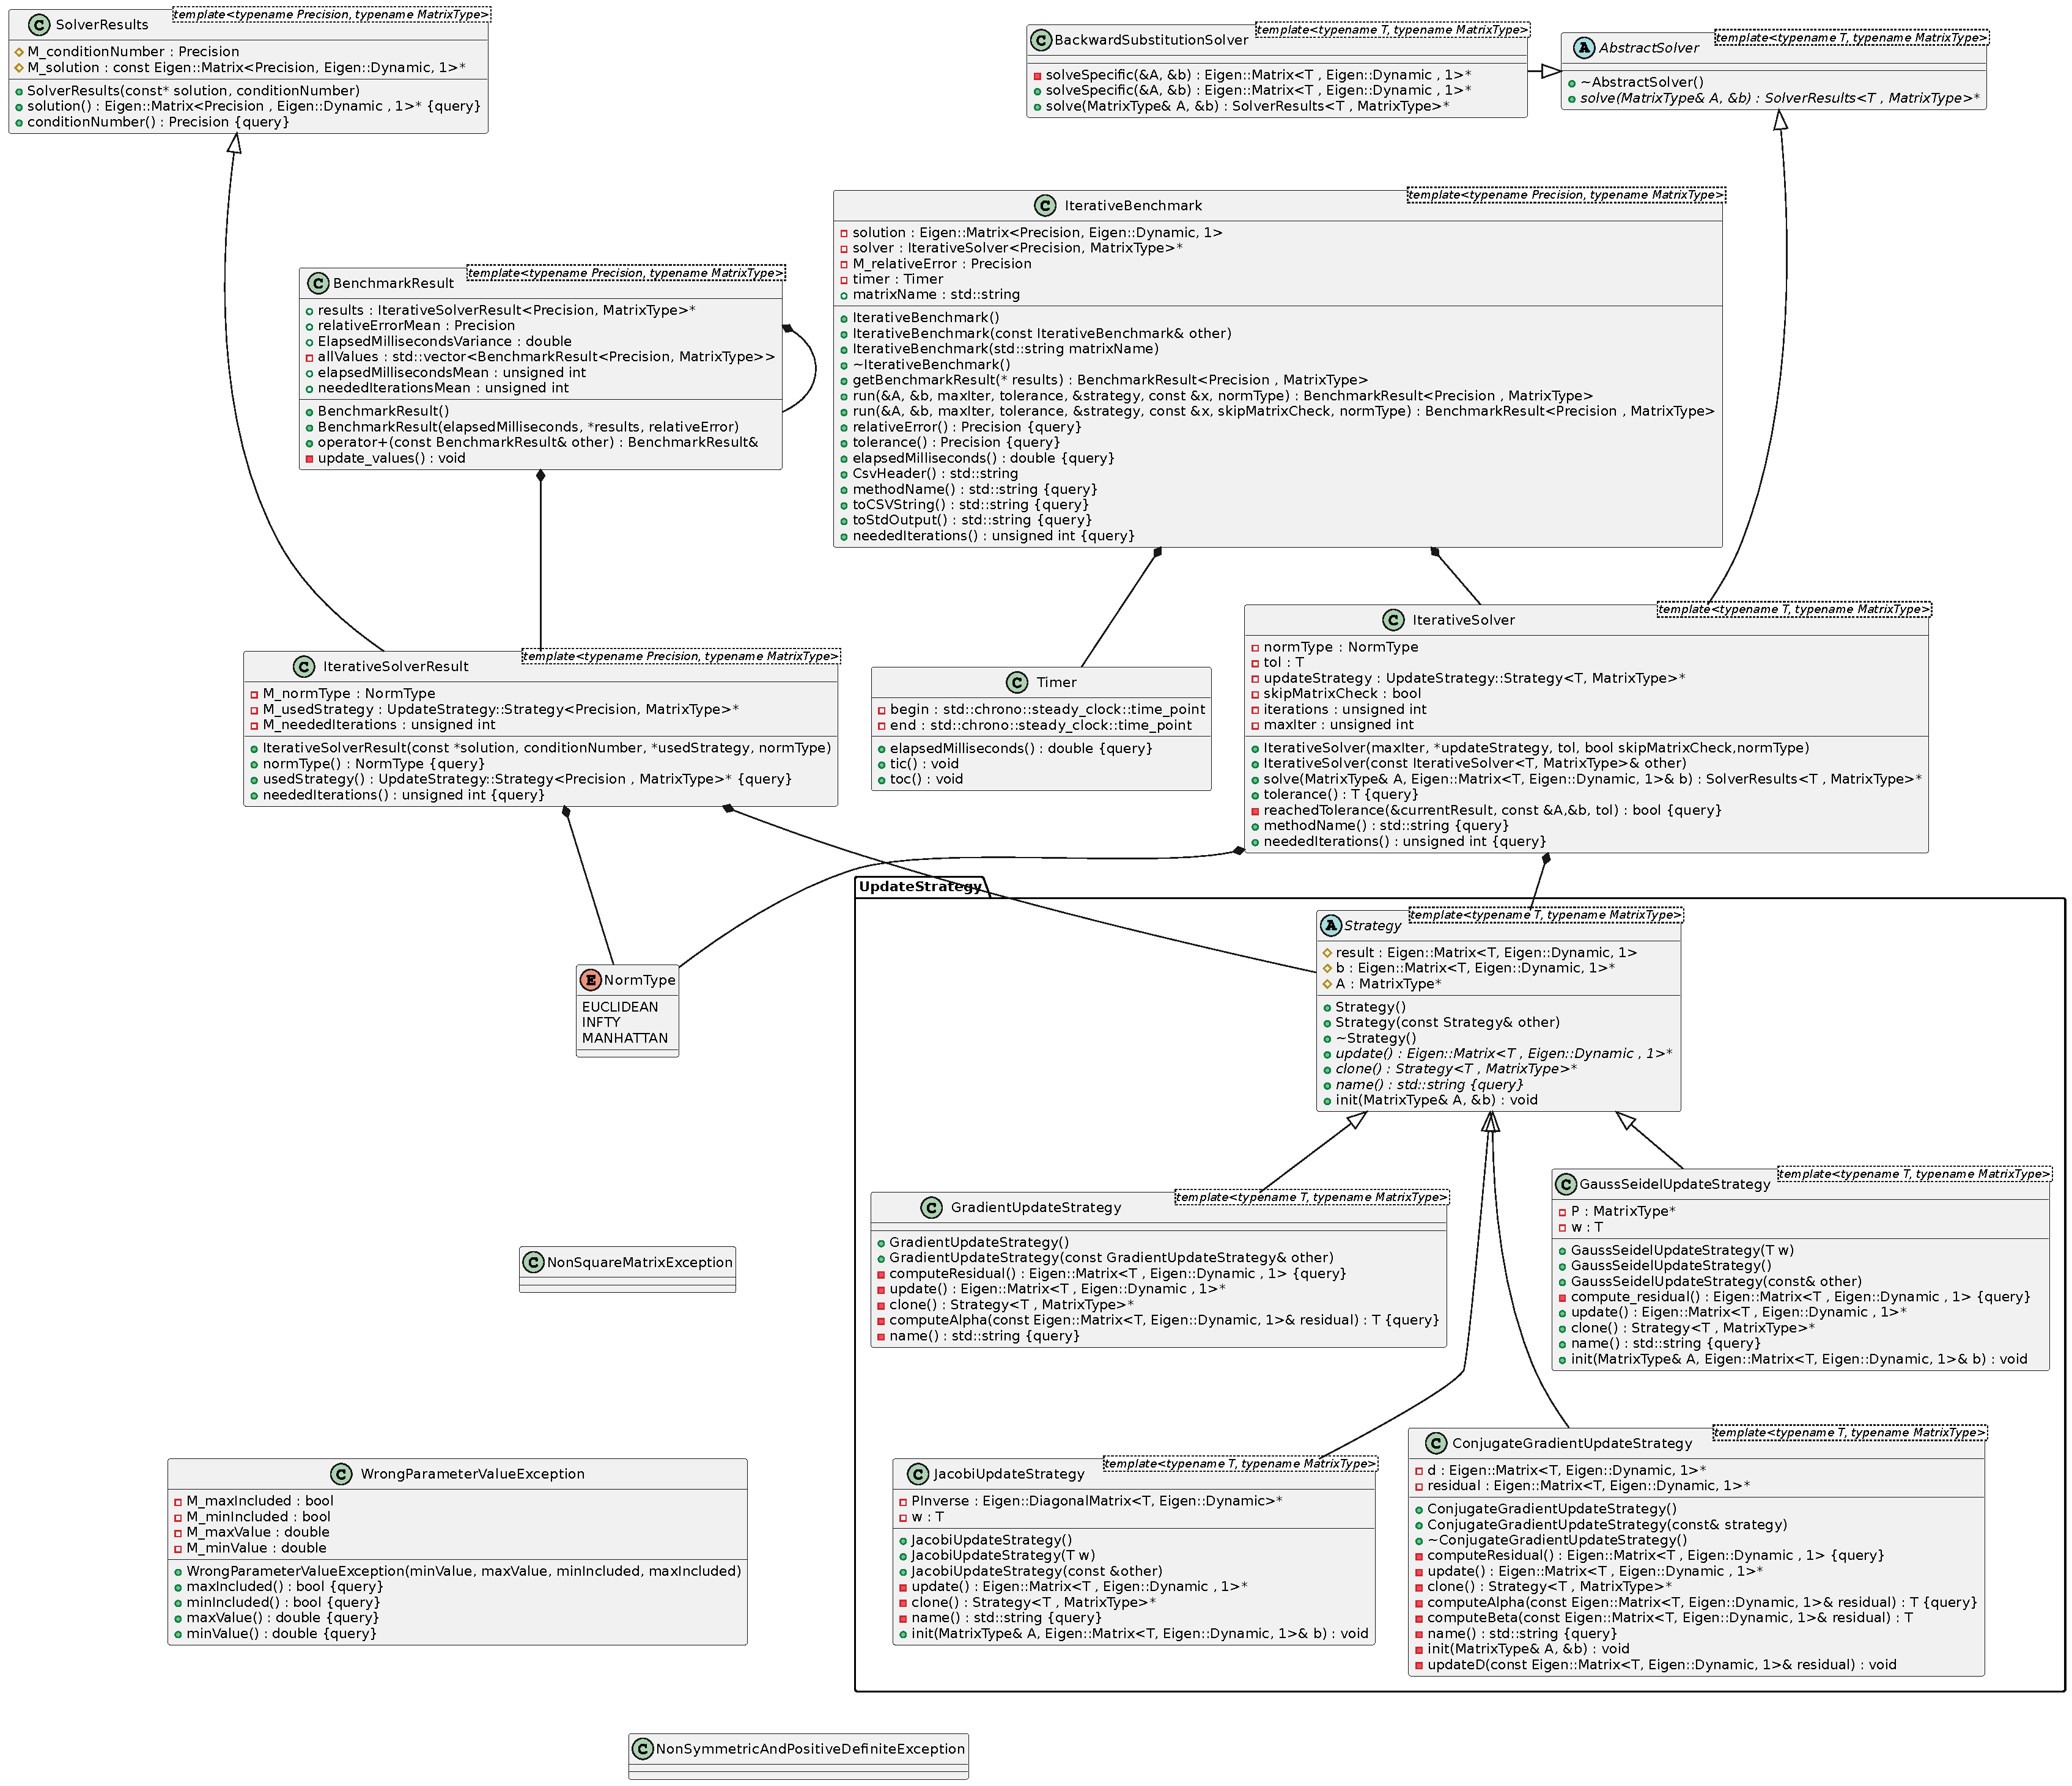
\includegraphics[width=\textwidth]{figures/libDiagram.pdf}
	\caption{Diagramma delle classi della libreria principale}
	\label{fig:libdiagram}
\end{figure}

\subsection{Applicazione da riga di comando} \label{sec:cli}
Questo sottoprogetto è molto piccolo, di fatto contiene una cli che accetta due sotto-comandi passati come stringhe:

\begin{enumerate}
	\item \path{solve}, che permette di specificare il percorso relativo ad una matrice da risolvere, applicandone i test creati.
	\item \path{test}, attraverso il quale è possibile eseguire i test su tutte le varie matrici di benchmark. È importante notare che, nel caso di test, le matrici devono trovarsi nella cartella \path{../Matrices/}.
\end{enumerate}

È importante notare che, a entrambi i comandi, si possono passare dei parametri utili a modificare il comportamento del solver. Nello specifico, sono presenti i seguenti:

\begin{itemize}
	\item \path{--jacobiW} indica il parametro $\omega$ per il metodo di Jacobi;
	\item \path{--gaussW} si riferisce al parametro $\omega$ per Gauss-Seidel;
	\item \path{--skipMatrixCheck} è utile per specificare se non serve controllare che la matrice data in input sia simmetrica e definita positiva;
	\item \path{--norm} permette di definire che tipo di norma usare nel controllo di convergenza. Le opzioni possibili sono \path{eucledian}, \path{manhattan} e \path{infinity}.
\end{itemize}

Per mantenere una coerenza tra i sottoprogetti, i test richiamano un header comune, il \path{runner.h}, il quale esegue le chiamate alla libreria sottostante e ne riporta i benchmark. Essendo in comune tra i progetti, esso è stato posto nella cartella principale, piuttosto che nella sottocartella \path{cli/}.


\subsection{Applicazione GUI}
Abbiamo creato anche una piccola applicazione con interfaccia grafica usando il framework Qt \cite{Qt}. Questa permette di:
\begin{itemize}
	\item Selezionare il file contenente la matrice de coefficienti
	\item Regolare i parametri $\omega$ per i metodi di Jacobi e Gauss-Seidel;
	\item Selezionare il tipo di norma da calcolare in fase di controllo della convergenza. Le scelte possibili sono euclidea, manhattan e infinito;
	\item Decidere di saltare il controllo che stabilisce se la matrice è simmetrica e definita positiva\footnote{Questa opzione può tornare utile per eventuali benchmark. Infatti, questo controllo richiede diverso tempo e rischia di nascondere le differenze tra i vari metodi in termini di tempo, soprattutto per matrici relativamente piccole};
	\item Visualizzare i risultati dei metodi sotto forma di tabella e di grafici che mostrano l'errore relativo e i tempi in funzione della tolleranza, raggruppati per metodo (Figura \ref{fig:ui:output}).
	\item Esportare i risultati in formato CSV.
\end{itemize}

Oltre a queste funzionalità, l'applicazione GUI mostra a schermo una finestra di avviso nel caso in cui l'inverso del  numero di condizionamento stimato sia troppo vicino a 0, al fine di informare l'utente di possibili errori molto alti nella risoluzione del sistema.

\begin{figure}%
	\centering
	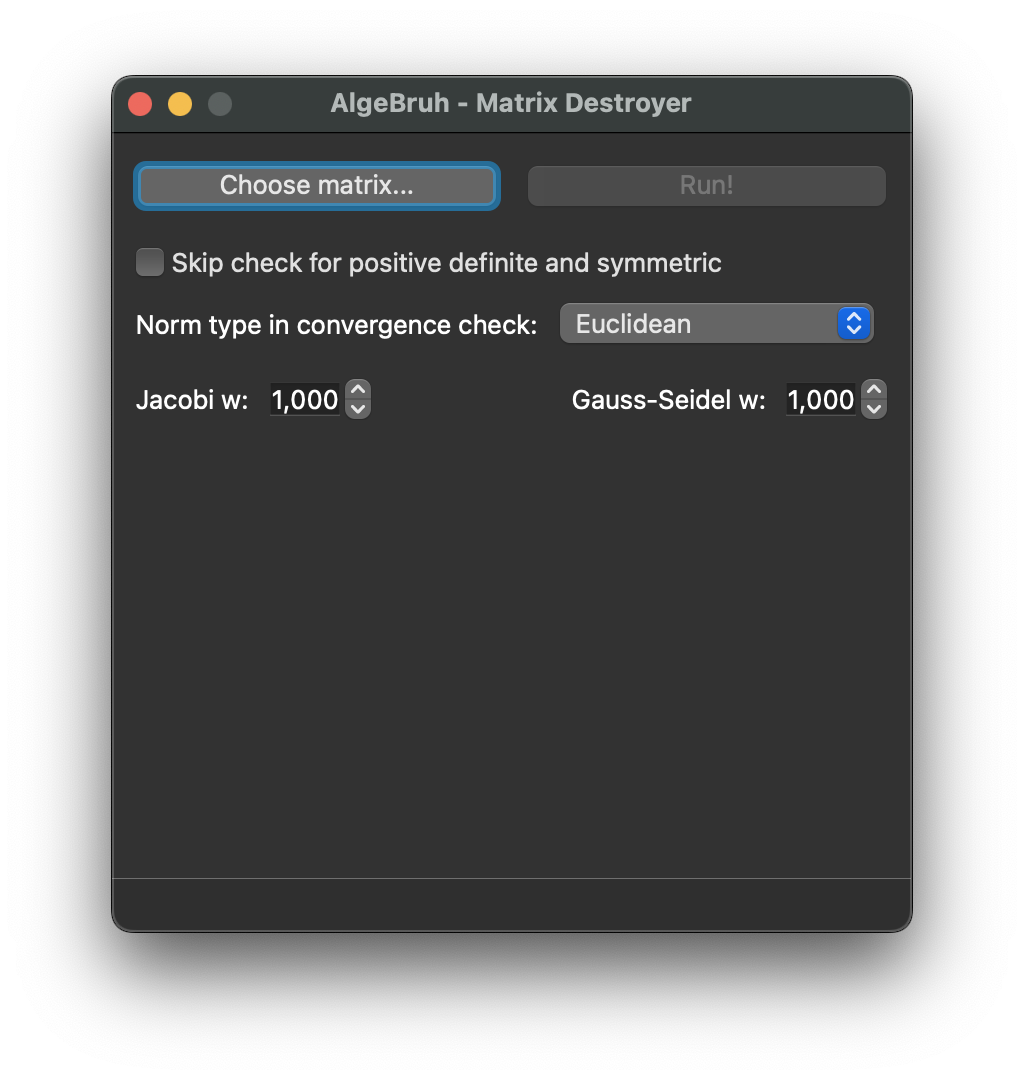
\includegraphics[width=0.5\textwidth]{figures/UI/main.png}
	\caption{Schermata iniziale dell'applicazione}%
	\label{fig:ui:main}%
\end{figure}

\begin{figure}%
	\centering
	\subfloat[\centering  Tabella riassuntiva]{{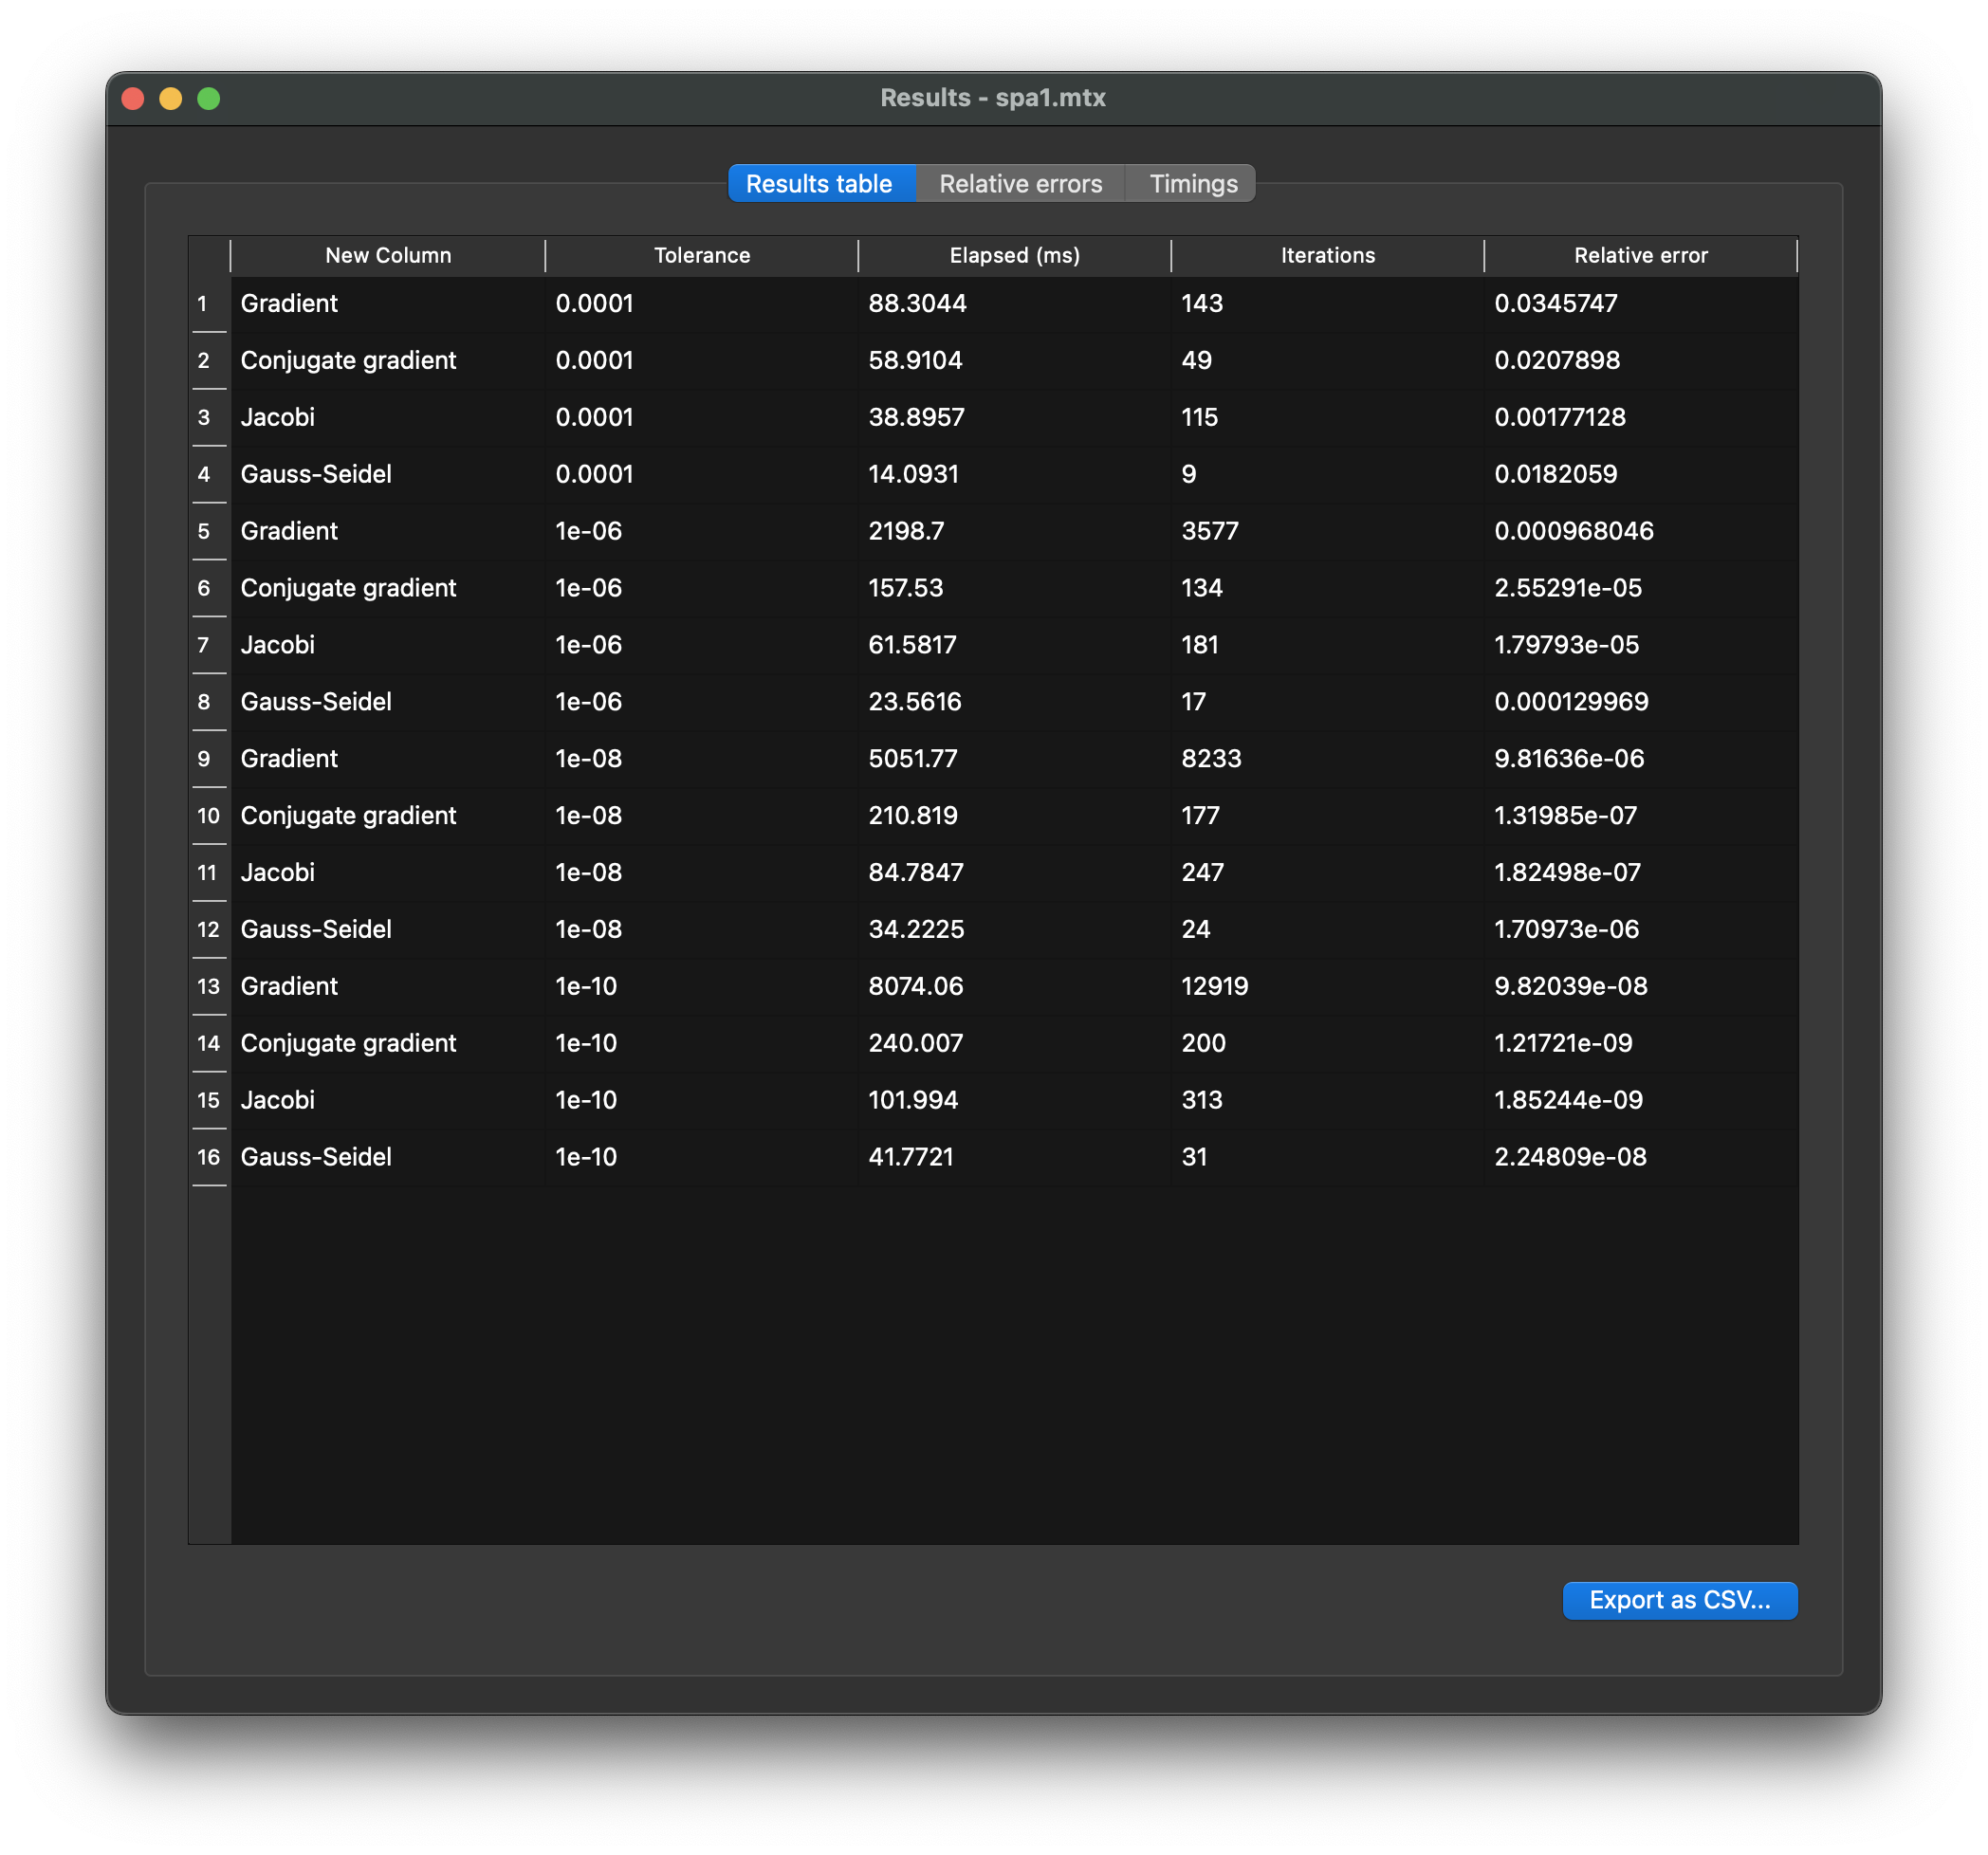
\includegraphics[width=0.45\textwidth]{figures/UI/table} }}%
	\qquad
	\subfloat[\centering Grafico tolleranza / tempi]{{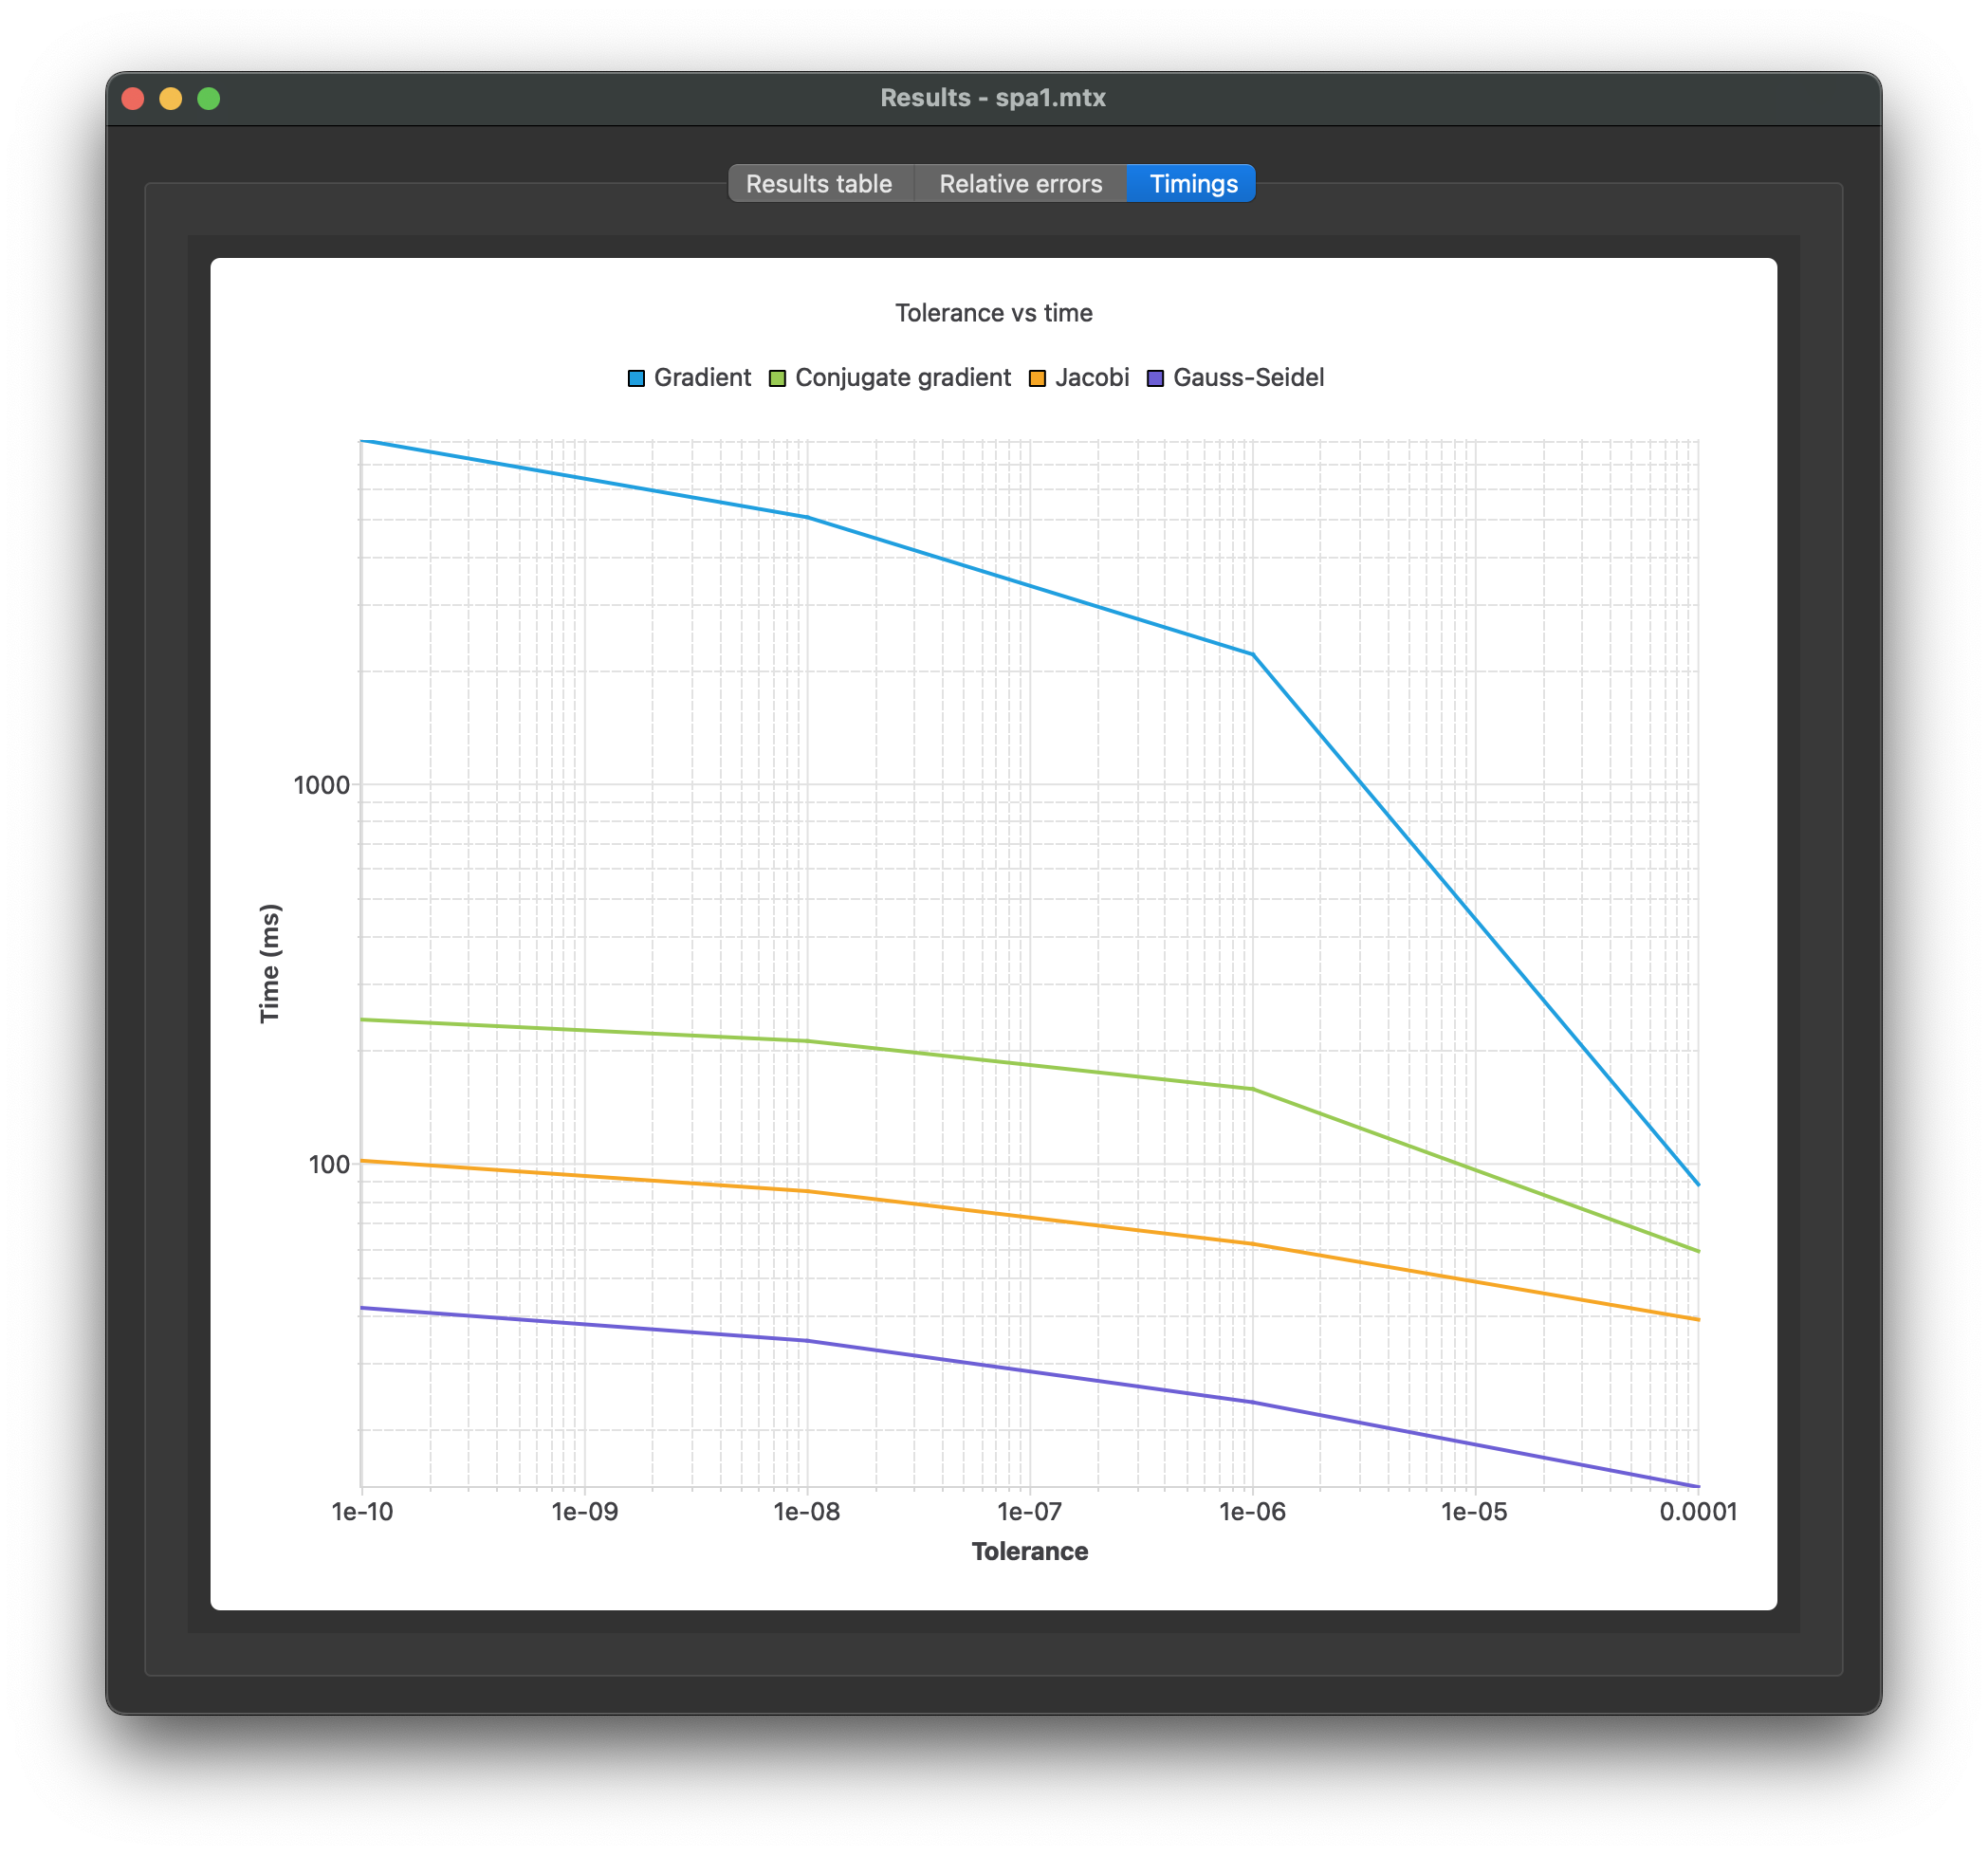
\includegraphics[width=0.45\textwidth]{figures/UI/chart} }}%
	\caption{Esempi di output prodotti dall'applicazione Qt}%
	\label{fig:ui:output}%
\end{figure}

Come per il progetto da riga di comando, questo è un eseguibile che effettua un linking statico verso la libreria, restando dunque un progetto separato da un punto di vista logico.
	\section{Features}

Nello sviluppo della libreria sono state introdotte un insieme di funzionalità aggiuntive, oltre alla possibile interazione tramite cli o GUI, quelle riguardanti unicamente l'implementazione della libreria sono illustrate di seguito:

\begin{itemize}
	\begin{item}
		\textbf{Controllo della matrice}: Prima di risolvere il sistema lineare si possono eseguire una serie di controlli sulla matrice, infatti per la corretta convergenza dei metodi iterativi è necessario che la matrice sia simmetrica e definita positiva.
	\end{item}
	\begin{item}
		\textbf{Stima del numero di condizionamento}: Assieme ai precedenti controlli, abbiamo deciso di calcolare un'approssimazione del numero di condizionamento della matrice dei coefficienti. Essa si basa sulla stima della norma 1 della sua inversa, senza l'effettiva inversione della matrice, attraverso il metodo di Hager \cite{hager, hager2}.
		
		Grazie a questa stima è possibile calcolare il condizionamento di $A$ attraverso la formula:
		$$ cond(A) = \|A\|_1  \|A^{-1}||_1$$
			
			\end{item}
	\begin{item}
		\textbf{Parametri dei metodi rilassati}: La libreria accetta i parametri $\omega$ per i metodi rilassati di Jacobi e Gauss-Seidel.
	\end{item}
	\begin{item}
		\textbf{Selezione della norma}: Possibilità di specificare una determinata norma da usare nel criterio di arresto del metodo iterativo. Le possibili norme impostabili sono: Euclidea, Manhattan e infinito.
	\end{item}
	\begin{item}
		\textbf{Forward substitution}: Abbiamo implementato la Forward substitution, iterando solamente sugli elementi presenti nella matrice. In questo modo è stato possibile sfruttare tale metodo per risolvere la matrice triangolare inferiore prodotta dall'algoritmo di Gauss-Seidel.
	\end{item}
	\begin{item}
		\textbf{Modularità}: Il formato della matrice é stato reso indipendente dalla risoluzione, infatti nella libreria è possibile specificare, come parametro templato, la tipologia di matrice da risolvere. Gli algoritmi implementati sono generici, in modo tale da per poter gestire entrambi i formati in modo flessibile.
	\end{item}
	\begin{item}
		\textbf{Tolleranza}: Il valore di tolleranza viene passato alla libreria per impostare l'approssimazione da raggiungere prima di arrestare il metodo iterativo.
	\end{item}

    \begin{item}
        \textbf{Eliminazione dei commenti}: I file .mtx potrebbero contenere dei commenti, in questa particolare estensione (.mtx) ogni riga di commento inizia con il carattere "\%". Abbiamo, dunque, fatto in modo che se presenti, i commenti vengano ignorati, così da evitare errori di importazione.
    \end{item}

\end{itemize}
	\section{Analisi e benchmark}

Per verificare che i metodi si comportassero in maniera corretta, abbiamo provato ad eseguire da interfaccia grafica una serie di test.
Le seguenti analisi nascono dai dati ricavati dall'esecuzione dei quattro metodi iterativi, i parametri considerati sono: \textit{tolleranza utilizzata} durante la fase di risoluzione, il \textit{tempo di esecuzione espresso in millisecondi}, il \textit{numero di iterazioni} effettuate per arrivare all'output, l'\textit{errore relativo} della soluzione ottenuta in relazione a quella di partenza e il \textit{nome della matrice risolta}. Il fine è quello di avere un'idea molto generale sul funzionamento dei metodi sui vari tipi di matrici.

\paragraph{Tolleranza vs errore relativo}
Abbiamo pensato di mettere in relazione l'errore relativo e la tolleranza utilizzata in fase di risoluzione dei quattro metodi a paragone; l'obiettivo è stabilire in che modo, al variare della tolleranza, il valore dell'errore relativo dei metodi potrebbe differire. In Figura \ref{fig:tolerrmat} e \ref{fig:tolerrmet} sono presenti i grafici relativi alla relazione tra tolleranza ed errore, raggruppati, rispettivamente, per matrici e per metodi.



\begin{figure}%
	\centering
	\subfloat{{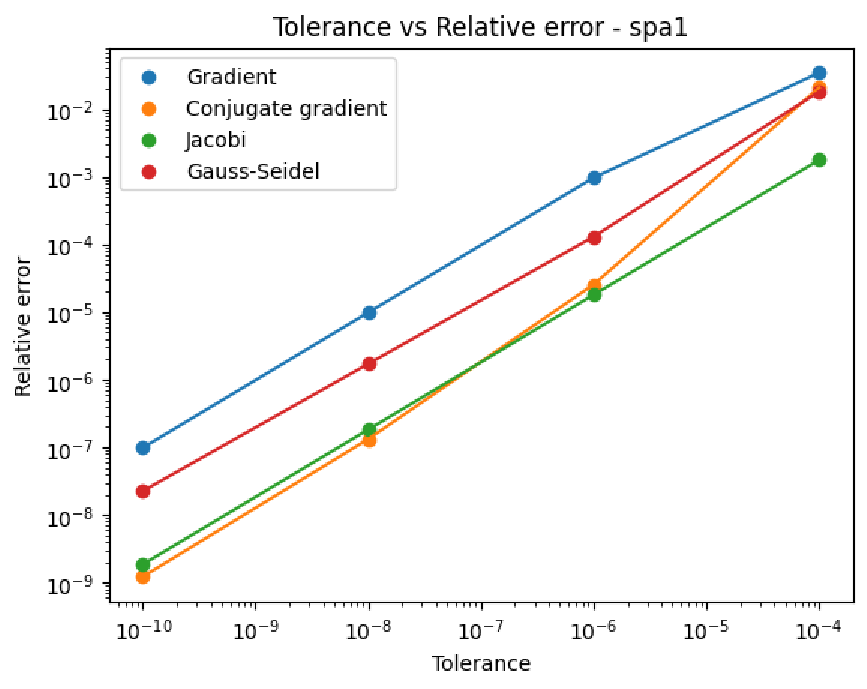
\includegraphics[width=0.40\textwidth]{figures/Tolerance vs Relative error/Difference between the 4 methods/spa1.pdf} }}%
	\subfloat{{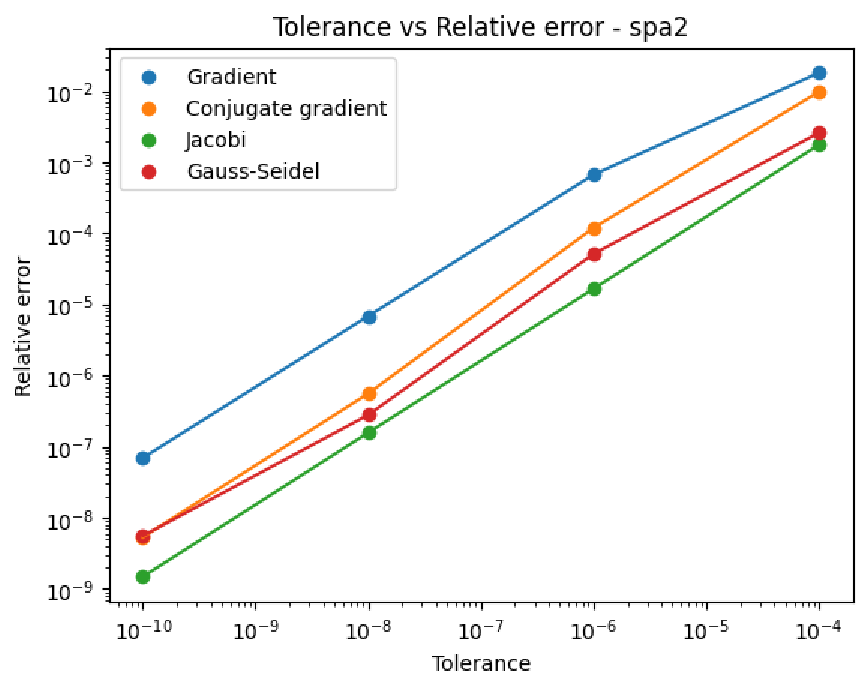
\includegraphics[width=0.40\textwidth]{figures/Tolerance vs Relative error/Difference between the 4 methods/spa2.pdf} }}%
	\qquad
	\subfloat{{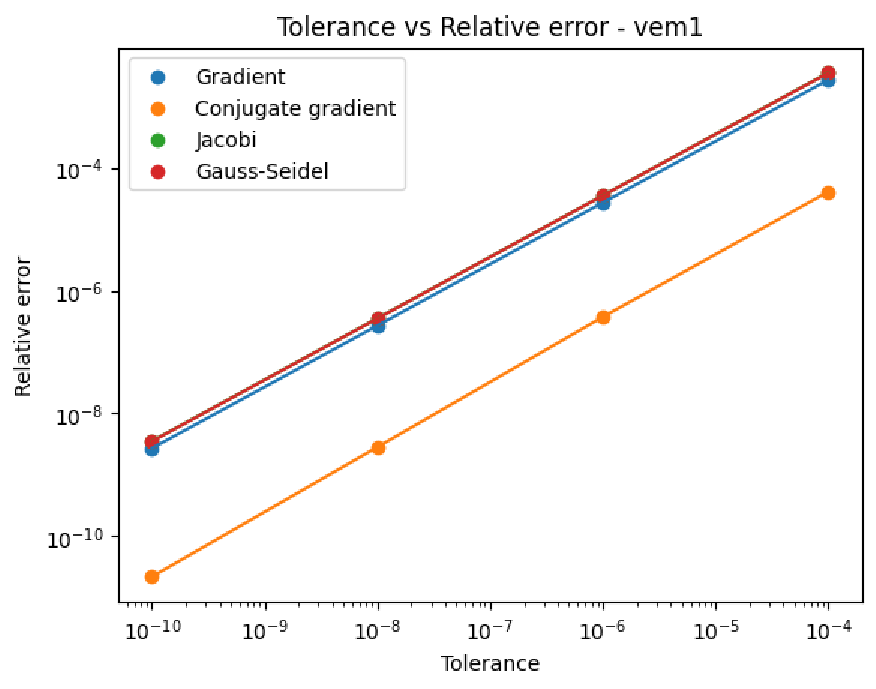
\includegraphics[width=0.40\textwidth]{figures/Tolerance vs Relative error/Difference between the 4 methods/vem1.pdf} }}%
	\subfloat{{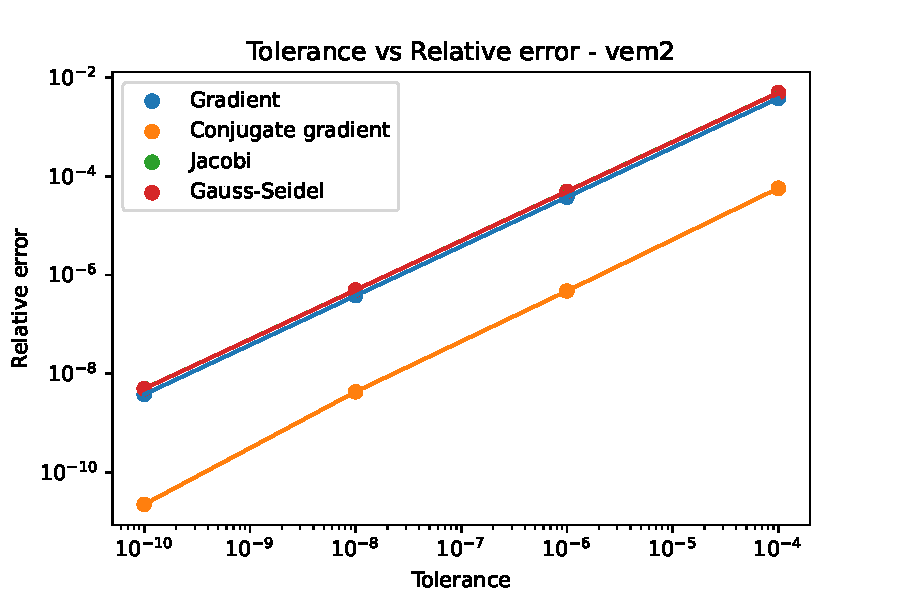
\includegraphics[width=0.40\textwidth]{figures/Tolerance vs Relative error/Difference between the 4 methods/vem2.pdf} }}%
	\caption{Grafici tolleranza / errore relativo sulle varie matrici di benchmark}%
	\label{fig:tolerrmat}
\end{figure}


\begin{figure}%
	\centering
	\subfloat{{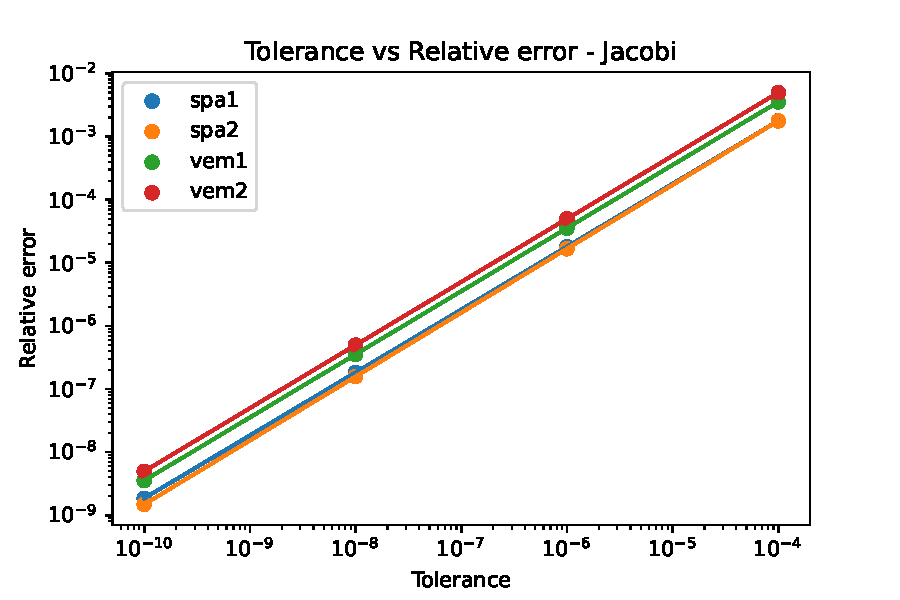
\includegraphics[width=0.40\textwidth]{figures/Tolerance vs Relative error/Difference between the 4 matrices on the same method/Jacobi.pdf} }}%
	\subfloat{{\includegraphics[width=0.40\textwidth]{figures/Tolerance vs Relative error/Difference between the 4 matrices on the same method/Conjugate Gradient.pdf} }}%
	\qquad
	\subfloat{{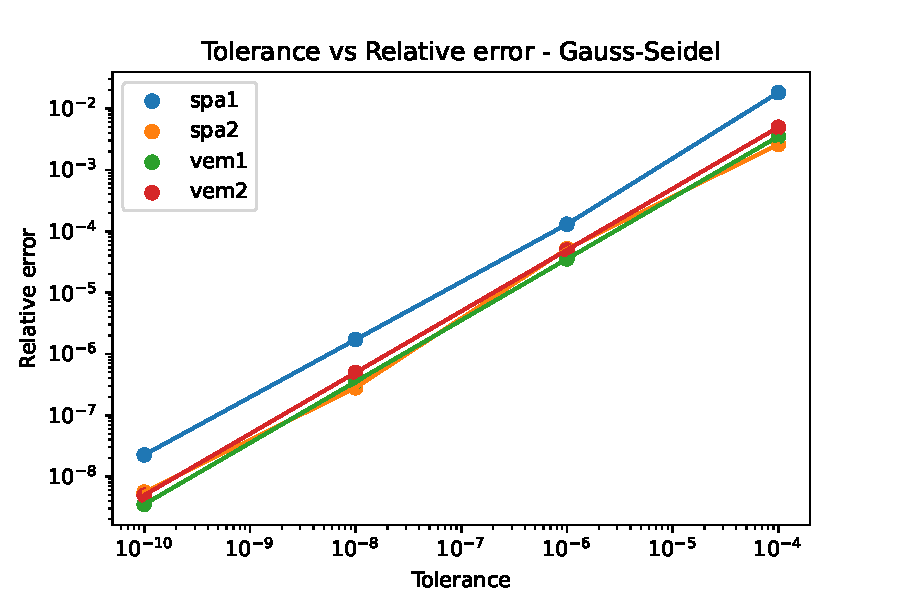
\includegraphics[width=0.40\textwidth]{figures/Tolerance vs Relative error/Difference between the 4 matrices on the same method/Gauss-Seidel.pdf} }}%
	\subfloat{{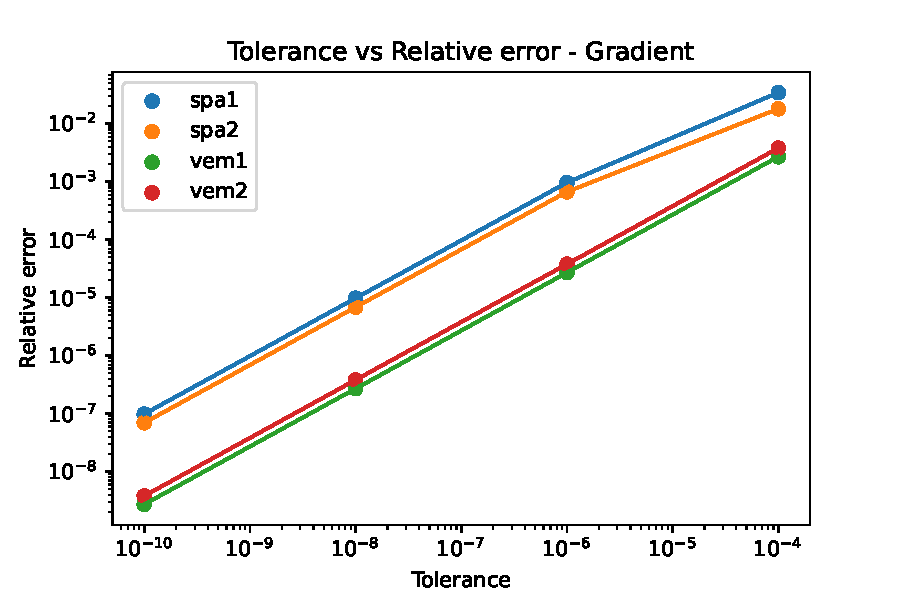
\includegraphics[width=0.40\textwidth]{figures/Tolerance vs Relative error/Difference between the 4 matrices on the same method/Gradient.pdf} }}%
	\caption{Grafici tolleranza / errore relativo rispetto i singoli metodi}%
	\label{fig:tolerrmet}
\end{figure}
%Immagine tolerance-relative_error, spa1, difference between the 4 methods
%Immagine tolerance-relative_error, spa2, difference between the 4 methods
%Immagine tolerance-relative_error, vem1, difference between the 4 methods
%Immagine tolerance-relative_error, vem2, difference between the 4 methods


Osservando i grafici, l'incremento dell'errore relativo è direttamente proporzionale alla crescita della tolleranza utilizzata durante l'esecuzione dei quattro metodi. Il risultato è ragionevole, così come indicato al capitolo \ref{tol/time, diff methods}, all'aumentare della tolleranza il criterio di arresto sarà meno restrittivo, portando ad una soluzione meno accurata, ergo ad un aumento dell'errore relativo.

\paragraph{Tolleranza vs tempo trascorso}\label{tol/time, diff methods}


\begin{figure}%
	\centering
	\subfloat{{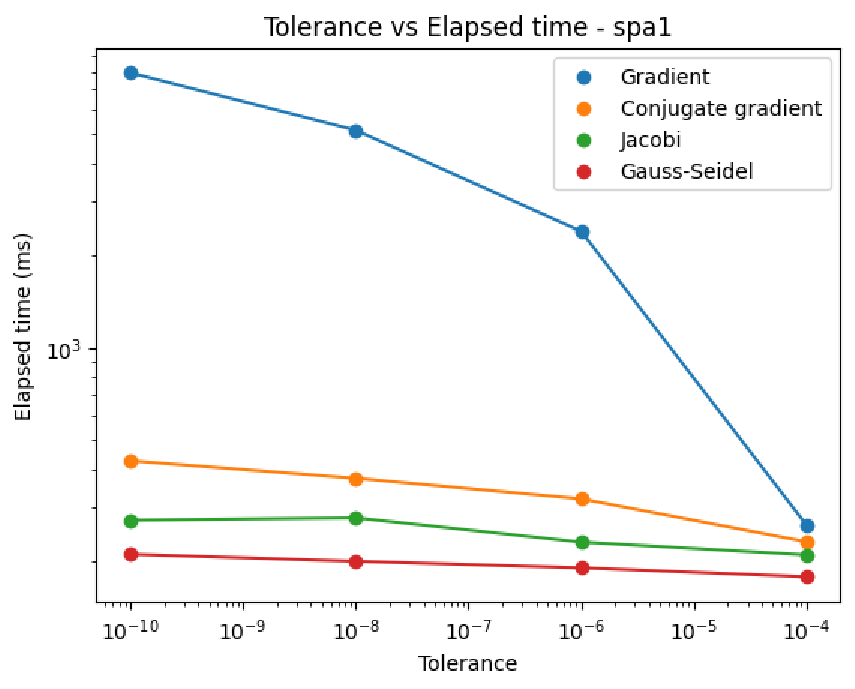
\includegraphics[width=0.40\textwidth]{figures/Tolerance vs Elapsed time/Difference between the 4 methods/spa1.pdf} }}%
	\subfloat{{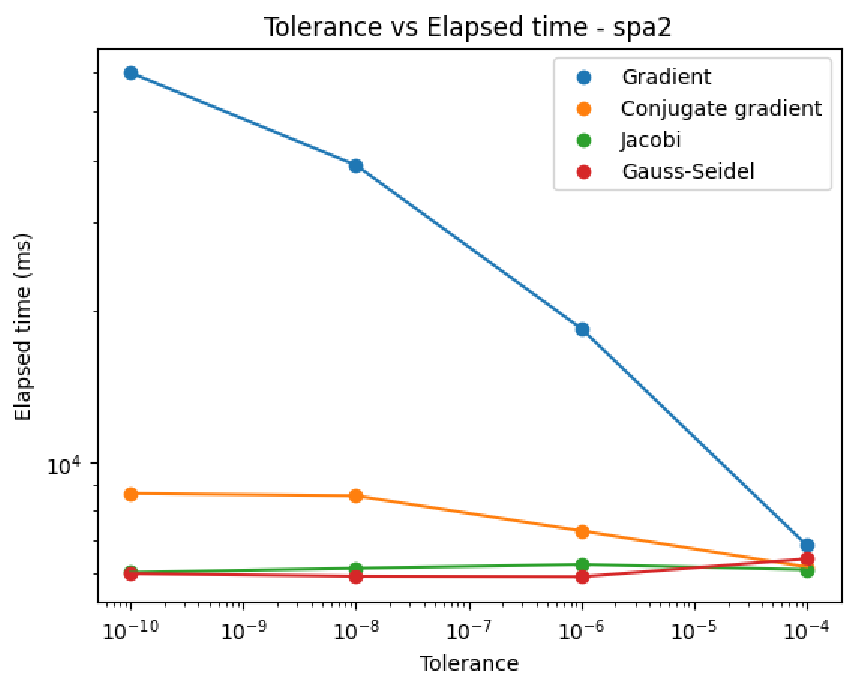
\includegraphics[width=0.40\textwidth]{figures/Tolerance vs Elapsed time/Difference between the 4 methods/spa2.pdf} }}%
	\qquad
	\subfloat{{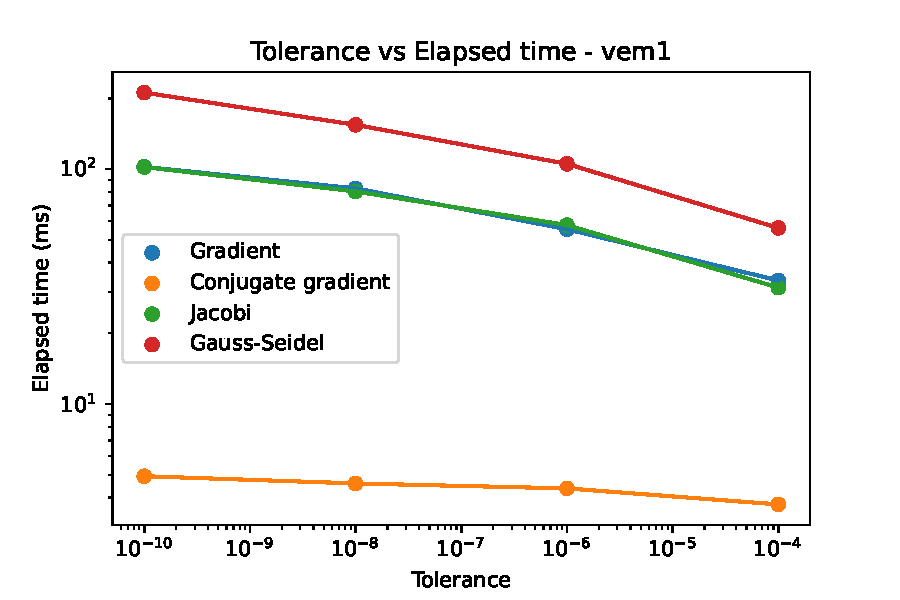
\includegraphics[width=0.40\textwidth]{figures/Tolerance vs Elapsed time/Difference between the 4 methods/vem1.pdf} }}%
	\subfloat{{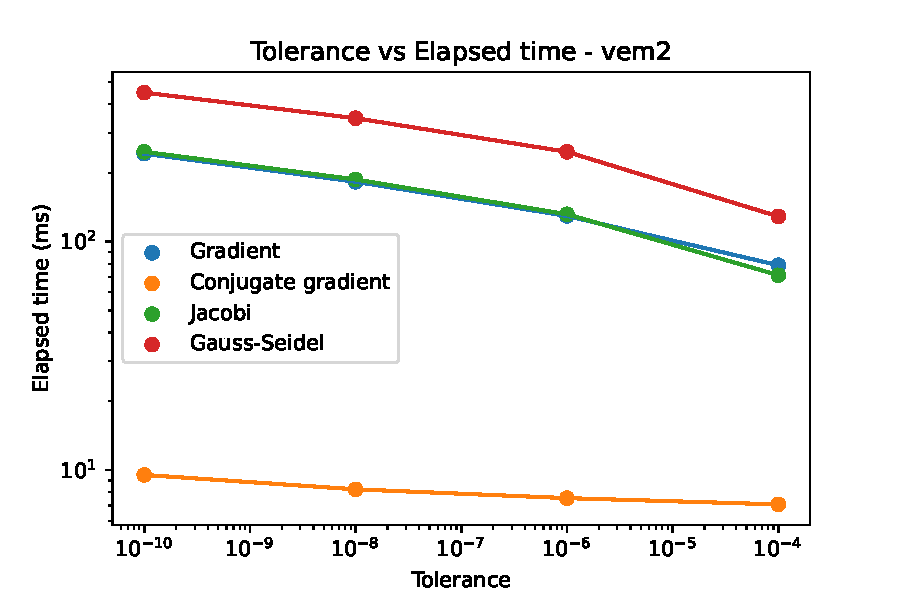
\includegraphics[width=0.40\textwidth]{figures/Tolerance vs Elapsed time/Difference between the 4 methods/vem2.pdf} }}%
	\caption{Grafici tolleranza / tempi sulle varie matrici di benchmark}%
	\label{fig:toltimemat}
\end{figure}

\begin{figure}%
	\centering
	\subfloat{{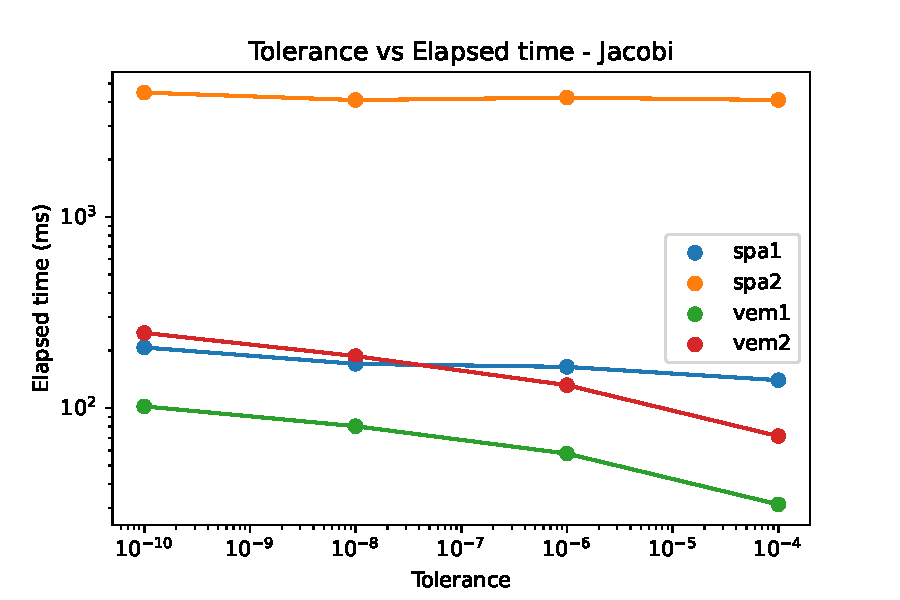
\includegraphics[width=0.40\textwidth]{figures/Tolerance vs Elapsed time/Difference between the 4 matrices on the same method/Jacobi.pdf} }}%
	\subfloat{{\includegraphics[width=0.40\textwidth]{figures/Tolerance vs Elapsed time/Difference between the 4 matrices on the same method/Conjugate Gradient.pdf} }}%
	\qquad
	\subfloat{{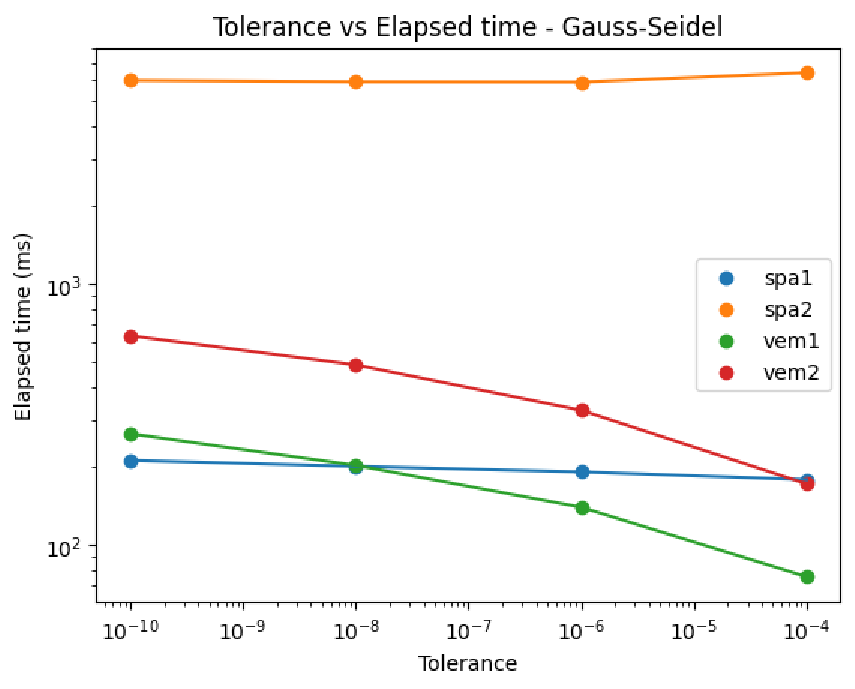
\includegraphics[width=0.40\textwidth]{figures/Tolerance vs Elapsed time/Difference between the 4 matrices on the same method/Gauss-Seidel.pdf} }}%
	\subfloat{{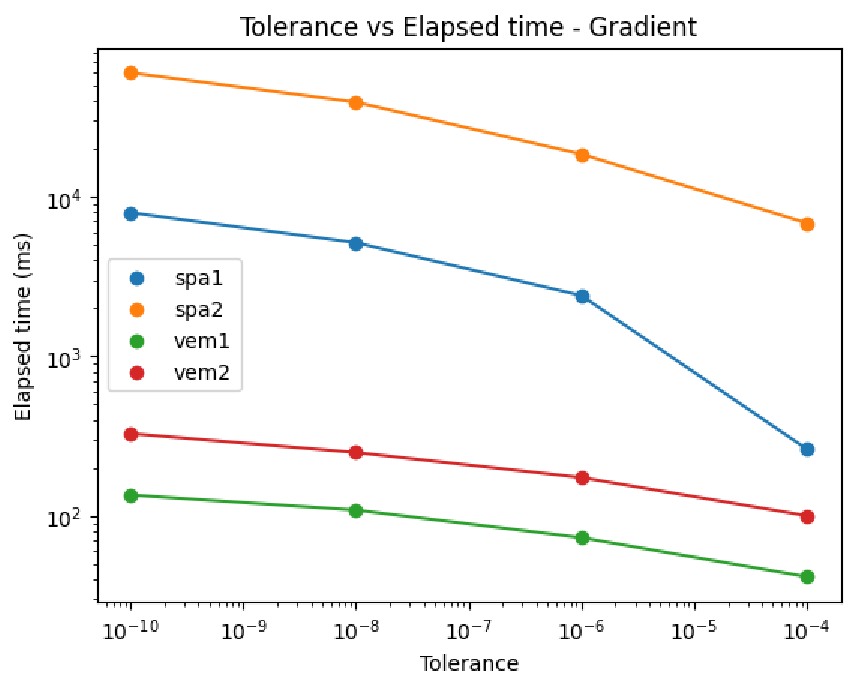
\includegraphics[width=0.40\textwidth]{figures/Tolerance vs Elapsed time/Difference between the 4 matrices on the same method/Gradient.pdf} }}%
	\caption{Grafici tolleranza / tempi rispetto i singoli metodi}%
	\label{fig:toltimemet}
\end{figure}
%Immagine tolerance-elapsedTime, spa1, difference between the 4 methods
%Immagine tolerance-elapsedTime, spa2, difference between the 4 methods

Nelle Figure \ref{fig:toltimemat} e \ref{fig:toltimemet} sono rappresentati i grafici relativi all'andamento del tempo rispetto alla tolleranza, raggruppati rispettivamente per matrice e per metodo.
Gauss Seidel è l'algoritmo che per le matrici relativamente dense, surclassa ogni altro metodo. Quando si passa a matrici estremamente sparse, come \path{vem1} e \path{vem2}, l'algoritmo che si comporta meglio sembra essere, invece, il gradiente coniugato.

Dai grafici si evince immediatamente che, all'aumentare della tolleranza, il tempo di esecuzione di ogni algoritmo tende a calare. Questa tendenza è più che ragionevole dato che, al calare della tolleranza, il criterio di arresto diventa più permissivo.
Tuttavia, è anche importante notare che, a differenza dell'errore relativo, il tempo di esecuzione dei vari metodi sembra poco sensibile sensible alla tolleranza selezionata; inoltre, l'andamento tra le due misure sembra dipendere pesantemente dal tipo di matrice, per ogni metodo. Questo potrebbe suggerire che ogni metodi funzionimeglio su un determinato tipo di matrice, anche se non abbiamo abbastanza dati per estrarre delle conclusioni. Questa osservazione è basata soprattutto dai grafici rappresentanti i tempi di Gauss-Seidel e di Jacobi: \path{vem1} e \path{vem2} sono matrici estremamente sparse, con una percentuale di elementi non nulli inferiore all'1\%, mentre \path{spa1} e \path{spa2} hanno una percentuale di elementi diversi da zero che si aggira attorno al 18\%: entrambi i metodi riescono ad abbassare visibilmente i tempi per le matrici molto sparse, mentre, nel caso della più dense, questo rimane più o meno invariato. Questa caratteristica, ovviamente, potrebbe dipendere anche da altri fattori non analizzati, come la qualità dei numeri presenti all'interno delle matrici.


%%%%%%%%%%%%%%%%%%%%%%%%%%%%%%%%%%%%%%%%%%%%%%%%%%%%%%%%%%%%%%%%%%%%%%%%%%%%%%%%%%%%%%%%%%%%%
%%%%%%%%%%%%%%%%%%%%%%%%%%%%%%%%%%%%%%%%%%%%%%%%%%%%%%%%%%%%%%%%%%%%%%%%%%%%%%%%%%%%%%%%%%%%%
%%%%%%%%%%%%%%%%%%%%%%%%%%%%%%%%%%%%%%%%%%%%%%%%%%%%%%%%%%%%%%%%%%%%%%%%%%%%%%%%%%%%%%%%%%%%%

%Immagine tolerance-elapsedTime, spa1, difference between the 4 matrixes on the same method
%Immagine tolerance-elapsedTime, spa2, difference between the 4 matrixes on the same method
%Immagine tolerance-elapsedTime, vem1, difference between the 4 matrixes on the same method
%Immagine tolerance-elapsedTime, vem2, difference between the 4 matrixes on the same method




	\FloatBarrier
	\newpage
	\printbibliography
\end{document}
	